\documentclass[twocolumn]{article}

%% Language and font encodings
\usepackage[english]{babel}
\usepackage[utf8]{inputenc}
\usepackage{csquotes}
\bibliographystyle{unsrt}
\usepackage{booktabs}

\usepackage{tabu}
\usepackage[T1]{fontenc}

%% Sets page size and margins
\usepackage[a4paper,top=2cm,bottom=2cm,left=3cm,right=3cm,marginparwidth=1.75cm]{geometry}

%% Useful packages
\usepackage{amsmath}
\usepackage{graphicx}
%\usepackage{apacite}
\usepackage[colorinlistoftodos]{todonotes}
\usepackage[colorlinks=true, allcolors=blue]{hyperref}

\title {Project: Recommender machine for movies}
\author{B. Shadrack Jabes}
\date{\it{\today}}

\begin{document}
\maketitle

\section{Introduction}
The aim of this project is to implement collabortive filter machine learning algorithm which when applied on a dataset of movie ratings can recommend a user movies that they would like to watch.  The dataset consists of 943 users, who have rated movies that they have watched on a scale of 1 to 5. There are about 1682 movies the users have watched in total. 
I compute the collaborative filetering cost function and its gradient and then learn the parameters for collaborative filering. Using this leanrned set of parameters I intend to recommend movies to the respective users.

\section{Dataset: Movie ratings}
Every user may not have watched all the movies and rated them. So we have a dataset of two variables here: 1. $Y$ and 2. $R(i,j)$ (1682 x 943). Here, the matrix $R(i,j)$ is zero but takes a value 1 if the $j^{th}$ has provided a rating on the $i^{th}$ movie he/she has watched. The rating the user has provided on the scale of  1 to 5 is contained in the Y (1682 x 943) matrix.
           \begin{figure}
                \centering
                \includegraphics[clip=true,trim=0cm 0cm 0cm 0cm,width=8cm]{../r_ratings_movies_users.ps}\\
                        \caption{The ratings of the movies by different users.}
                \label{fig:dataset}
                \end{figure}
\section{Collaborative filtering learning algorithm}
\subsection{cost function}
In order to recommend movies using this algorithm, I consider a set of $n$ dimensional vectors $X = x^{(1)}...x^{(n_m)} and \theta^{(1)}...\theta^{(n_u)}$. Here $n_u$ and $n_m$ are the number of users and number of movies respectively. These parameters $X$ and $\theta$ when multiplies yields a polynomial $y_{prediction} = (\theta^(j))^Tx^{(i)}$. Using this model I predict the rating for the movie, $i$ by user $j$. The dataset provided contains a set of ratings by some users on some movies only. Given such a data the unknown parameter vectors $X$ and $\theta$ can be learned based on the best fit or the choice of parameters that minimizes the squared error.
\begin{align*}
	J(x^{(1)}...x^{(n_m)}, \theta^{(1)}...\theta^{(n_u)}) = \\\frac{1}{2}\sum_{(i,j);r(i,j)=1} ((\theta^(j))^Tx^{(i)} - y^{(i,j)})^2  \\+ \frac{\lambda}{2}\sum_{j=1}^{n_u}\sum_{k=1}^{n}(\theta_k^{(j)})^2 \\+ \frac{\lambda}{2}\sum_{i=1}^{n_m}\sum_{k=1}^{n}(x_k^{(j)})^2
\end{align*}
The first term of the above equation is the cost function and the second and third terms are the regularization of the cost function.
\subsection{gradient}
To extract the parameters that minimizes the cost I implement the regularization for the gradient.
\begin{align*}
	\frac{dJ}{dx_k^{(i)}} = \sum_{(i,j);r(i,j)=1} ((\theta^(j))^Tx^{(i)} - y^{(i,j)})\theta_k^{(j)} + \lambda x_k^{(i)}\\
	\frac{dJ}{d\theta_k^{(j)}} = \sum_{(i,j);r(i,j)=1} ((\theta^(j))^Tx^{(i)} - y^{(i,j)})x_k^{(i)} + \lambda \theta_k^{(j)}\\
\end{align*}
\section{Training the algorithm to recommend}
I have rated a set of movies and used the collaborative filter machine learning algorithm to recommend me a list of movies. The following is the movies that I rated and the recommendation by the algorithm (see figure \ref{fig:recommend}).
	   \begin{figure}[htbp]
                \centering
                \includegraphics[clip=true,trim=0cm 0cm 0cm 0cm,width=8cm]{../r_movie_rating_movie_recommended.ps}\\
                        \caption{Movies rated by me and the movies recommendation by the algorithm}
                \label{fig:recommend}
                \end{figure}
\section{Contribution}
I implemented the  collaborative filtering learning algorithm. To enhance the computational efficiency I have vectorized programming code.
\end{document}
